\documentclass[]{article}
\usepackage{graphicx}

%opening
\title{Solution for Problem Set D}
\author{}

\begin{document}
	
	\maketitle
	
	\section{Problem D1}
	\begin{itemize}
		\item[a] Hardware redundancy:
		\item[i]Static Hardware redundancy is based on voting. It uses the concept of fault masking and consists of a voter that forwards the majority vote of all inputs.
		\begin{figure}[h]
			\centering
			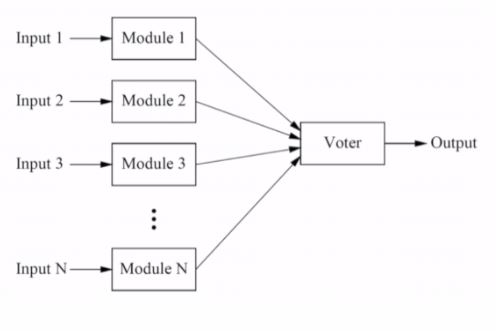
\includegraphics{Static}  
			\caption{Static hardware redundancy}
		\end{figure}
		
		
		Reliability of the voter is high because of low complexity.
		\item[ii] Dynamic hardware redundancy : Output of the module at any instance is determibed by only one module. Fault Detector is used in dymanic hardware redundancy which observes input and activates output of other module ("spare") if error observed.
		\begin{figure}[h]
			\centering
			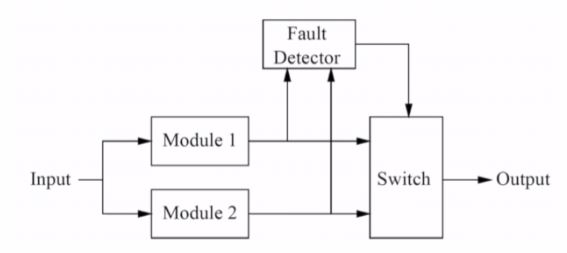
\includegraphics{Dynamic}  
			\caption{Dynamic hardware redundancy}
		\end{figure}
		\item[b] Setup chosen for each application
		\item[i]Dynamic hardware redundancy setup with two modules and one fault detector.\\Justification:Module is 98\% reliable upto 1 year. Hence chances of it's failure are very low. Module is used in mission only for 30mins after which it is replaced.In case one module fails  during the flight, fault is detected by the fault detector and output is switched to other module. Using static setup with 3 modules and one voter will lead to excess expenditure(since module costs significant amout of money) and size. Hence using dynamic hardware redundancy in this application is cost effective and also reliable.
		\item[ii]Static hardware redundancy setup with three modules and one voter.\\Justification:Module is 99.5\% reliable upto only 1 year whereas it is used in an application for 50 years. There are chances of the module becoming faulty after a period of time. Using 3 modules and a voter helps in masking the fault of one module. Also, since module is a part of a satellite, replacement of module if it becomes faulty is very difficult. Thus, taking into consideration the duraion of usage and difficulty of replacement of module, it is better to take majority vote out of the 3 modules. Hence static hardware redundancy is preferable.
		\item[iii]Dynamic hardware redundancy setup with two modules and one fault detector.\\Justification:Module is 99\% reliable upto 1 year and is used in an applicaiton which is not very critical. Also, it is checked for failures once a day when it may or may not be replace. If a module is faulty, fault detector will detect the fault and switch the output to other module. The faulty module can then be replaced during daily checking.  Using static setup with 3 modules and one voter will lead to excess expenditure(since module costs significant amout of money) and size.  Hence using dynamic hardware redundancy in this application is best solution.
	\end{itemize} 
	
\end{document}
